\section{RNN‑Transducer (RNN‑T)}

\begin{frame}[t,allowframebreaks]{RNN‑Transducer (RNN‑T): Overview}
    \textbf{RNN‑Transducer (RNN‑T)} is a sequence-to-sequence model widely used for end-to-end speech recognition. It extends the CTC (Connectionist Temporal Classification) approach by modeling both input and output dependencies:

    \begin{itemize}
        \item \textbf{Sequence-to-sequence model:} Maps input sequences (e.g., acoustic features) directly to output sequences (e.g., transcriptions).
        \item \textbf{End-to-end speech recognition:} Eliminates the need for separate components (like acoustic, pronunciation, and language models).
        \item \textbf{Extension of CTC:} 
            \begin{itemize}
                \setlength{\itemsep}{-0.5em}
                \item CTC models only input dependencies and assumes output tokens are conditionally independent.
                \item RNN-T models both input and output dependencies, allowing the prediction of each output token to depend on previous outputs.
            \end{itemize}
        \item \textbf{Key advantage:} Enables more accurate modeling of language and flexible alignments between input and output.
    \end{itemize}

    \begin{figure}[h]
        \centering
        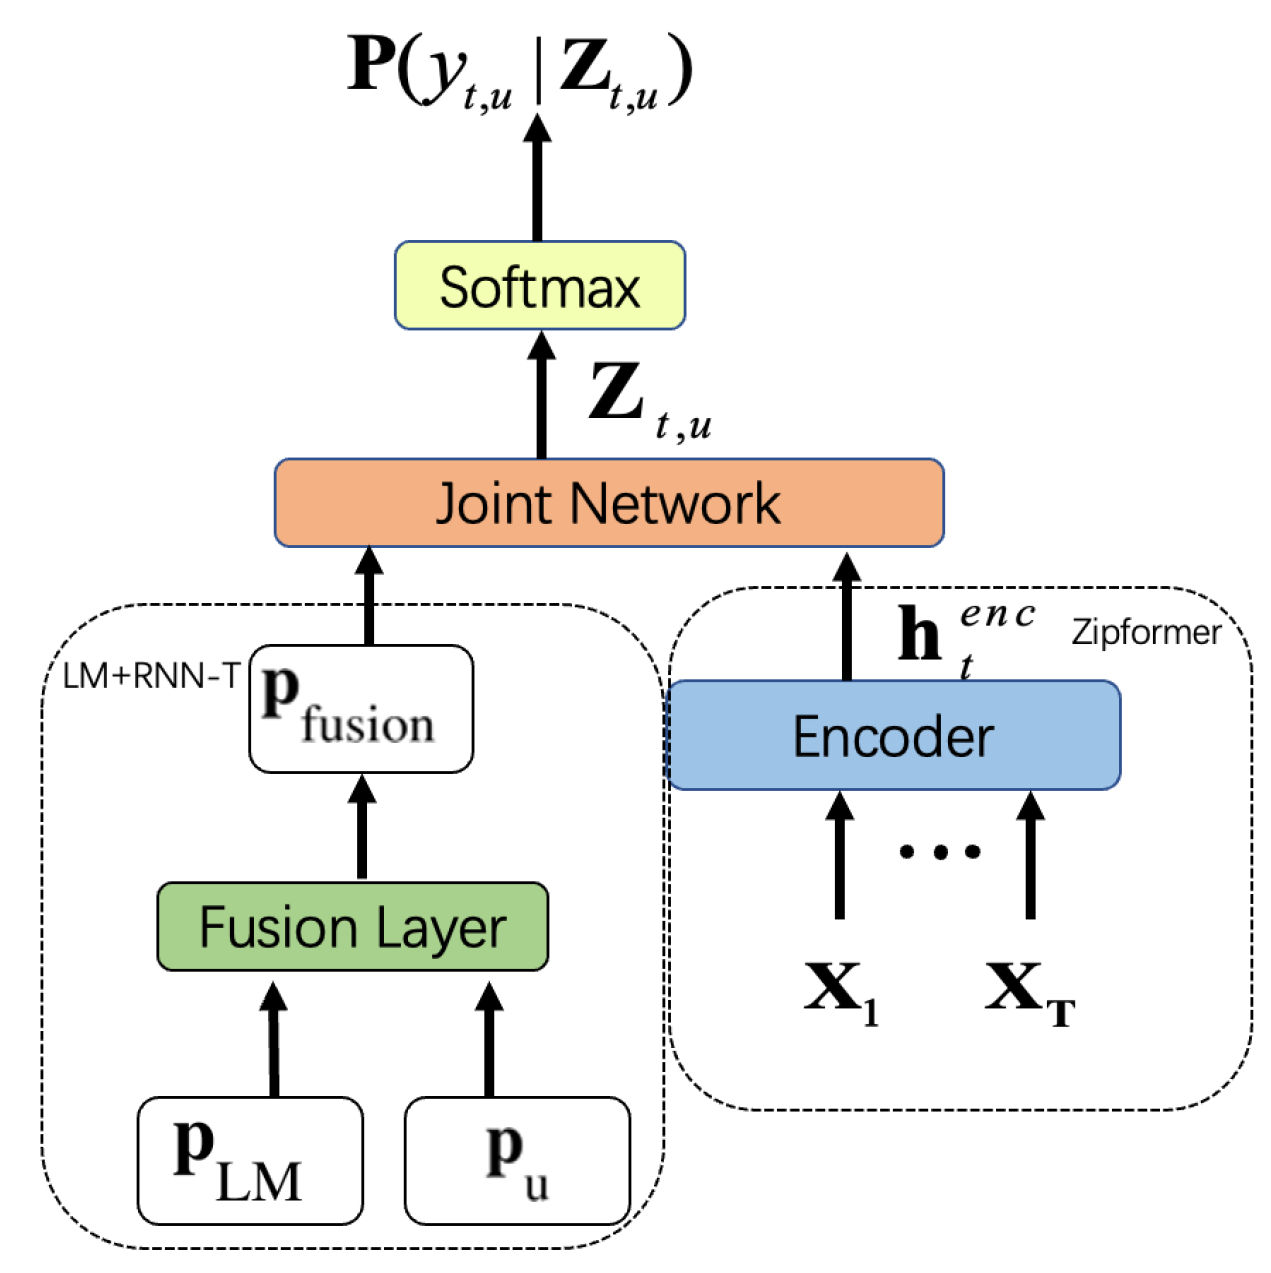
\includegraphics[width=\textwidth,height=0.8\textheight,keepaspectratio]{images/audio-nlp/rnnt_architecture.png}
        \caption*{RNN‑T Architecture: Encoder, Prediction Network, and Joint Network.}
    \end{figure}

    \framebreak

    \textbf{Architecture Components:}
    \begin{itemize}
        \item \textbf{Encoder:} Processes the input acoustic features and produces high-level representations.
        \item \textbf{Prediction Network:} Acts like a language model, conditioning on previous non-blank output tokens.
        \item \textbf{Joint Network:} Combines encoder and prediction network outputs to produce logits over the output vocabulary (including the blank symbol).
    \end{itemize}

    \begin{equation}
        \mathbf{h}_t = \text{Encoder}(\mathbf{x}_{1:t})
    \end{equation}
    \begin{equation}
        \mathbf{g}_u = \text{PredictionNetwork}(y_{1:u-1})
    \end{equation}
    \begin{equation}
        \mathbf{z}_{t,u} = \text{JointNetwork}(\mathbf{h}_t, \mathbf{g}_u)
    \end{equation}

    \framebreak

    \textbf{Loss Overview:}
    \begin{itemize}
        \item RNN‑T loss marginalizes over all possible alignments between input and output sequences.
        \item Similar to CTC, but allows for output dependencies.
        \item Computed efficiently using dynamic programming.
    \end{itemize}

    \begin{equation}
        \mathcal{L}_{\text{RNN-T}} = -\log \sum_{\pi \in \mathcal{A}(\mathbf{y}, T)} P(\pi | \mathbf{x})
    \end{equation}
    where $\mathcal{A}(\mathbf{y}, T)$ is the set of all valid alignments.

    \framebreak

    \textbf{Pros vs. CTC:}
    \begin{itemize}
        \item Models output dependencies (better language modeling).
        \item No need for external language model during inference.
        \item More flexible alignments.
    \end{itemize}

    \textbf{Cons vs. CTC:}
    \begin{itemize}
        \item More complex and computationally intensive.
        \item Harder to train and tune.
        \item Decoding is slower due to output dependencies.
    \end{itemize}
\end{frame}